%!TEX root = ../thesis_rui_almeida.tex
%%%%%%%%%%%%%%%%%%%%%%%%%%%%%%%%%%%%%%%%%%%%%%%%%%%%%%%%%%%%%%%%%%%%
%% 3_methods.tex
%% Rui V. Almeida's thesis file
%%
%% This chapter contains the methods presentations and discussion
%%%%%%%%%%%%%%%%%%%%%%%%%%%%%%%%%%%%%%%%%%%%%%%%%%%%%%%%%%%%%%%%%%%%
\chapter{Methods}
\label{cha:methods}

\todo[inline]{\textbf{\large{THIS CHAPTER WAS DIRECTLY PULLED FROM THE
TOMOSIM ARTICLE AND NEEDS A LOT OF WORK BEFORE IT IS COMPLETE.}}}

This chapter details the methods that were used trying to answer the
research questions that were determined in
Chapter~\ref{cha:introduction}. They reflect the three-pronged nature
of this whole work, detailing the design of the UAV system and its
projected features, the simulation software that was used to validate
the mathematical approach and to understand if this method would be able
to obtain a "spectral image" of a certain number of trace compounds in
a given region of the atmosphere, and finally, the experiment that was
designed and conducted to validate the measurement strategy on which
this system is based.

\section{The drone}%
\label{sec:the_drone}

Consider a drone equipped with a DOAS system and the ability to command
spectral acquisition. The spectral system cannot perform point
measurements, but only averaged measurements over a large region. This
makes drawing a twodimensional (eventually tridimensional) map of trace
polutants in a region an impossible task if one were to apply the
technique directly. One can, however, consider each spectral acquisition
as if it were a projection of the field of analysis. If this is the
case, then it should be possible to create that polutant map using
tomography. This immediately implies the need of an adequate trajectory.

This trajectory will have to encompass the whole area in study, and
movement within it must allow the equipment to perform all the
measurements at angles such that it is possible for the tomography
algorithm to reconstruct an image from the acquired data. As illustrated
by Figure~\ref{fig:trajectory_schematic}, movement within the trajectory
will go as follows:
\begin{itemize}
    \item Drone starts at a given point, which must be defined and
        known;
    \item Drone moves along a circumference, stopping at regular angular
        intervals, which are configured at scan time;
    \item On each of the stops, the drone points the spectral equipment
        at the center of the trajectory;
    \item Drone rotates. First to one side, then the other. Again on
        fixed intervals the drone stops rotation for a given period of
        time;
    \item During each rotation stop, the spectral equipment acquires
        data;
\end{itemize}

Each spectral measurement is approximated to a ray, and the set of rays
in each stop along the circumference is a fanbeam shaped projection. To
facilitate the resorting operation of the projections, the angular
interval between each stop is the same as the one between rays.

\begin{figure}
    \begin{subfigure}[t]{.49\textwidth}
    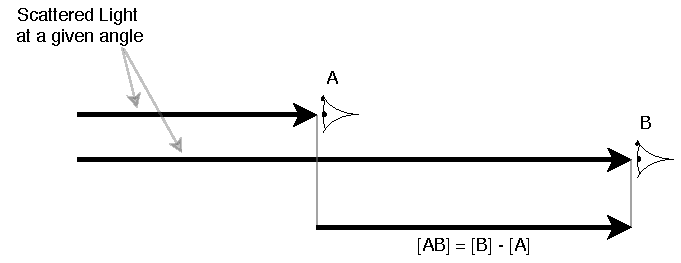
\includegraphics[width=\linewidth]{img/pdf/spectralMeasurementSketch.pdf}
    \caption{Measurement hypothesis: the number of molecules that
    interact with scattered light between A and B is the same as the
    subtraction of the number of molecules found to have interacted at A
    from the number of molecules found in B}
    \label{fig:measurement_hypothesis}
\end{subfigure}
\hfill
\begin{subfigure}[t]{.49\textwidth}
    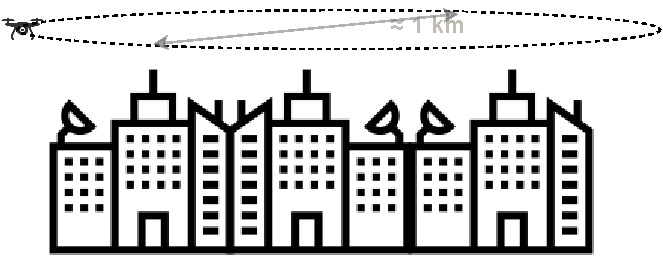
\includegraphics[width=\linewidth]{img/pdf/spectralMeasurementsFromTheSide.pdf}
    \caption{Measurement schematic representation: the drone covering
    an urban area of about 1 km in diameter.}
    \label{fig:measurements_from_the_side}
\end{subfigure}
\caption{Schematic representation of the spectroscopic principle and the
measurement strategy employed by this system.}
\label{fig:measurement_strategy_schematics}
\end{figure}

\section{The Simulator: TomoSim}%
\label{sec:the_simulator_tomosim}

\subsection{Tomographic Procedures}%
\label{sub:tomographic_procedures}

As discussed in Subsection~\ref{sub:measurement_trajectory}, the UAV's
trajectory and acquisition strategy generate what is treated
subsequently as a fanbeam geometry problem. Before reconstructing the
spectral image however, one must convert the continuous nature of the
natural space into a discrete model, which can be interpreted by the
computer, in the discretisation step. Siddon's algorithm is used for
this effect. It allows the calculation of the optical path for each ray
in a fan. More importantly, it returns the portion of these paths that
is in each "pixel". This is a very important piece of data, since it
will be assembled onto what is called the system matrix, which
fundamental for iterative reconstruction methods.

The most important part of the implementation of Siddon's algorithm in
what concerns this simulator is the determination of three starting
parameters: number of lines, line starting point (p1) and line finishing
point (p2). The first parameter is set by the number of pixels in the
phantom, which is a configurable parameter. p1 is also in part set by
the size of the phantom, but also depends on the projection angle. p2 is
algebrically calculated using the ray's slope to determine its line
equation and then some vector properties to find where this line
intersects the trajectory circumference, which becomes a matter of
solving a simple second degree equation after some algebric
manipulation. After these three parameters are completely determined,
discretisation of the field of analysis is achieved through a normal
implementation of Siddon's algorithm, as is described in
Section~\ref{sec:theoretical_background}.

With the space conveniently discretised, the routine starts
reconstructing the image from the generated projection data. Since no
actual measurements were conducted during the development of this
simulation, gas concentration was also simulated, as well as their
spatial distribution. Concentration values, which actually are column
density values, were chosen to be similar to the ones that can be found
in nature. Spatial distribution information is provided to the
simulation routine in a phantom form. In tomography, a phantom is an
artificial image that is used to test reconstruction algorithms. One of
the most commonly used phantoms in tomographic imaging is the
Shepp-Logan phantom (see Figure~\ref{fig:shepplogan}), which was
designed to mimic the human head structure. This phantom is very readily
available in the relevant literature and was therefore used for the
development of this simulation routine. The phantom's structure,
however, is not very adequate to one of atmospheric spectral imaging.
For this reason, the phantom presented in Figure~\ref{fig:new_phantom}
was designed.

\begin{figure}
    \centering
    \begin{subfigure}[t]{0.45\textwidth}
    \begin{center}
        
\includegraphics[width=\textwidth]{img/png/shepp_logan.png}
    \end{center}
    \caption{Shepp-Logan phantom, commonly used in medical imaging.}
    \label{fig:shepplogan}
    \end{subfigure}
    \hfill
    \begin{subfigure}[t]{0.45\textwidth}
    \begin{center}
        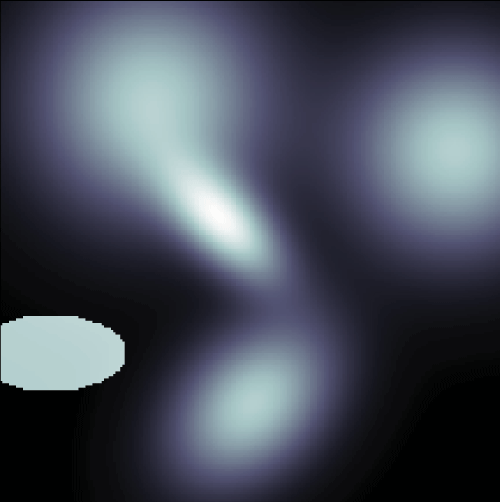
\includegraphics[width=\textwidth]{img/png/spectral.png}
    \end{center}
    \caption{New phantom, designed for spectroscopic analysis of
    atmopsheric trace gases.}
    \label{fig:new_phantom}
    \end{subfigure}
    \caption{Set of phantoms used for the Tomosim simulator.}
\end{figure}

In this simulation, the pixel value is related to the concentration of
the trace gas being sampled by using the projections themselves as
normalising units. Light enters the Region Of Interest at point P1 and
leaves at point P2. At the entrance point, light is simulated through
the use of a solar spectrum with no atmospheric contamination (see
~\cite{Kurucz1984}). The ROI is populated with the some concentration of
trace gases that one wants to simulate, distributed along one of the
phantom matrices that have been discussed. Pixel values in these
matrices are equated to molecule numbers.

When setup in this manner, one can simulate a detector \emph{looking}
from point P2 to point P1, and \emph{seeing} the contamination of the
solar spectrum by the trace gases in the phantom. The simulator then
applies the Siddon algorithm from P1 to P2 and thus calculates the
number of molecules traversed by each ray of light. All the numbers for
all the projections are then assembled onto a single matrix, the
sinogram. The optical lengths of each pixel for each ray are also stored
in the system matrix. In real life measurements, this process is
slightly more complicated, because the contamination at point P1 is not
known \emph{a priori}.

Reconstruction algorithms \emph{per se} only start at this point, in two
ways: iterative and analytical. For the latter, there is still an
intermediate step, in which the fanbeam sinogram collected by the device
is transformed into a parallel projection sinogram (pseudocode for this
transformation is shown in Algorithm~\ref{alg:resorting}). Iterative
algorithms, however, do not require this step, since they are mostly
independent of the problem's geometry~\cite{Defrise2003}.

After running the reconstruction, the simulator already provides a
twodimensional map of the trace gas in the ROI, but it lacks the numeric
values for the measured densities. The image matrix is, at this point, a
collection of 32 bit floating point numbers from 0 to 1. These numbers
can be normalised by running Siddon's algorithm again for a limited
number of projections, and equating calculated projections with the ones
that were acquired from the original phantom.

\section{The Experiment}%
\label{sec:the_experiment}

As stated in this chapter's introductory notes, this thesis main body of
work revolves around two base assumptions, our hypothesis. The first
one, about the information capturing by the idealised system, was
addressed in lkjashdkjh~\todo{reference the correct subsection after
merging with the mac branch}. The second, more physical in nature, is
the subject matter of this section. Our hypothesis states that the light
absorption between points $A$ and $B$ (let's call it $A_{AB}$) should be
equal to the difference of the absorptions in $A$ and $B$. We can write
this, in a \emph{Lambertian} manner as in
Equation~\ref{eq:lambertian_hypothesis}.

\begin{equation}
    \label{eq:lambertian_hypothesis}
    I_B = I_A \cdot \exp \bigg[-AB \cdot \sum_i \sigma_{ABi} \cdot
    c_{ABi}\bigg]
\end{equation}

This is to say that the light intensity reaching point $B$ is given by
the intensity reaching $A$, exponentially decreased by the absorbers at
interval $AB$. The intensities at $A$ and $B$ are written as in
Equation~\ref{eq:intensityAtAAndB}.

\begin{equation}
    \begin{aligned}
        \label{eq:intensityAtAAndB}
        I_B = I_0 \cdot \exp \bigg[ -L_B \cdot \sum_i \sigma_{Bi} \cdot
        c_{Bi} \bigg]\\
        I_A = I_0 \cdot \exp \bigg[ -L_A \cdot \sum_i \sigma_{Ai} \cdot
        c_{Ai} \bigg]
    \end{aligned}
\end{equation}

If we join all this information in the same expression, the equation is
transformed into its final form, presented in
Equation~\ref{eq:hypothesis_final_form}.

\begin{equation}
    \small
    \label{eq:hypothesis_final_form}
    I_0 \cdot \exp \bigg[ -L_B \cdot \sum_i \sigma_{Bi} \cdot
            c_{Bi} \bigg] = I_0 \cdot \exp \bigg[ -L_A \cdot \sum_i \sigma_{Ai} \cdot
            c_{Ai} \bigg] \cdot \bigg[-AB \cdot \sum_i \sigma_{ABi} \cdot
            c_{ABi}\bigg]
\end{equation}

Equation~\ref{eq:hypothesis_final_form} can be greatly simplified: we
take the natural logarithm of both sides and we state that $\sum_i
\sigma_{Xi} \cdot c_{Xi} = S_i$. These operations result in the
simplified form of Equation~\ref{eq:final_form_simplified}.

\begin{equation}
    \label{eq:final_form_simplified}
    L_B \cdot S_B = L_A \cdot S_A + L_{AB} \cdot S_{AB}
\end{equation}

Now, $L_X \cdot S_X$ can be thought of as the wavelength dependent light
absorption in path $X$. In this case, the wavelength interval is always
the same. We can therefore conclude that, theoretically, our
hypothesis is valid: light absorption between points $A$ and $B$ can be
expressed in terms of the absorption on both these points and
corresponds to their difference.

Although mathematically this seems clear-cut, in the real world things
can become more problematic, since we have to deal with the
imperfections that characterise a real physical system. Noise,
instrumental limitations, adverse environmental effects, etc.. The
experiment we describe in the next few paragraphs aimed at determining
target trace gas concentration in a set analysis field. This field is
dimension-wise compatible with those that would be employed in the final
working system. The experiment geographic information is presented in
Figure~\ref{fig:experiment_map}.

\begin{figure}[htpb]
    \centering
    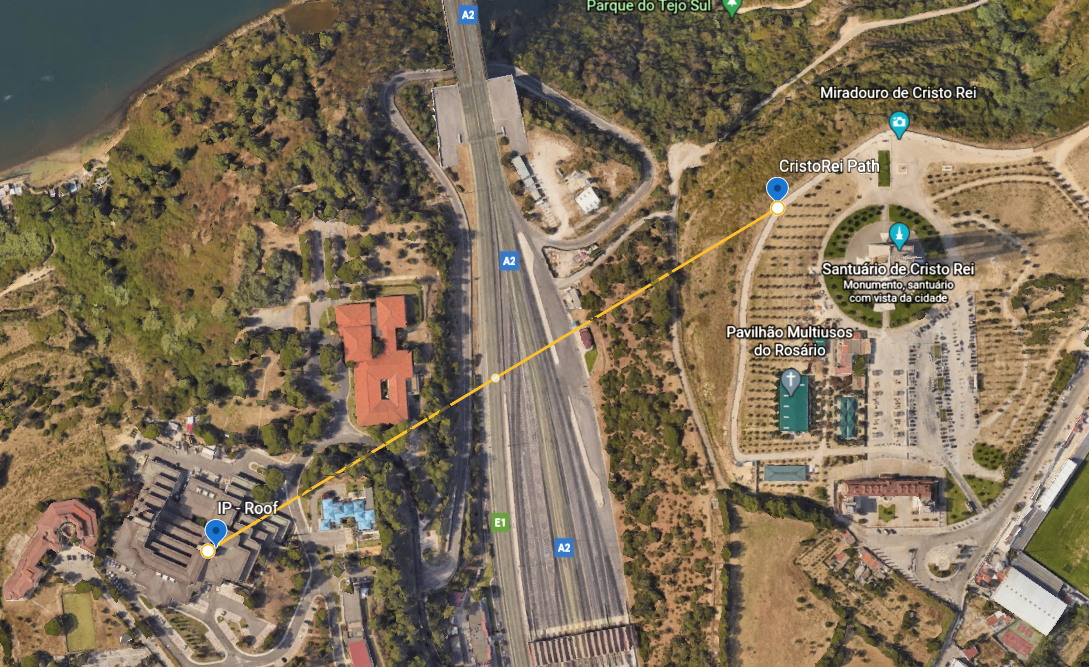
\includegraphics[width=0.8\linewidth]{img/png/experimentMap.png}
    \caption{Location of observer points for the physical experiment.}
    \label{fig:experiment_map}
\end{figure}
